
We built it and it works! We call it STS: the SDN Troubleshooting Simulator.
Our code is publicly available.\\

%We simulate the entire network, including hosts and
%switches, in a single-threaded process, and running the controllers in
%individual virtual machines that are
%bootstrapped from a static snapshot (including random number generator
%seeds, \etc{}). The switches connect to the controllers as if they were true
%network devices, such that the controllers believe they are configuring a true
%network. The simulator interposes on all communication channels,
%allowing it to proceed with the system execution in
%lock step~\cite{Dunlap:2002:REI:844128.844148}:
%pausing the controller VMs between each logical timestep and delaying messages
%arbitrarily. The simulator then reproduces the external inputs from the log.
%For example, link failures are reproduced by disconnecting the edge in
%the simulated network.

A few implementation details:

\begin{itemize}
\item Exactly what we log (not dataplane packets!)
\item Note that it's OK if there are slight re-orderings in the internal
events during replay: we have buffers.
\item Lightweight deterministic replay: we instrument gettimeofday() and getrand() for some controllers, since it's easy, and it helps us deal with timeouts properly.
\item When we alter history, we make a best-effort guess for the
instrumentation. For example, if the altered execution asks for more rands/dates than we recorded initially. Just feed it more rands generated on-the-fly, and assume somewhat equidistant (in time) requests for datetime.
\end{itemize}

OK, so what are the ways developers and operators can put sts into action?

\subsection{Replayable Traces}
\begin{itemize}
\item Forget about the algorithm for a second.
\item This tool gives us replayable traces.
\item Much better than status quo useful for dev mailing list help (e.g. Murphy and NOX bugs on nox-dev)
\end{itemize}

\subsection{Testing}
%\colin{Use Amin's quote from ONS to motivate utility of simulator}
%\colin{Amin Vahdat:
%I understand another key benefit of SDN/OpenFlow is being able to play with a
%lot of "what if" scenarios to enable you to fine-tune the network before going
%live.
%
%Exactly. So one of the key benefits we have is a very nice emulation and
%simulation environment where the exact same control software that would be
%running on servers might be controlling a combination of real and emulated
%switching devices. And then we can inject a number of failure scenarios under
%controlled circumstances to really accelerate our test work.}
\begin{itemize}
\item Simulator gives you complete control over orderings, message drops, node failures, etc.
\item It also gives us a total ordering of internal/input events
\item Can play with tricky cases interactively
  \begin{itemize}
  \item because of our lightweight instrumentation, traces generated through interactive exploration can be played back at a much faster speed.
  \end{itemize}
\item Can also automatically generate random inputs $\rightarrow$ replayable integration tests!
\item Can accumulate a library of tests to run on other controllers.
\item frees up developers to be more agile in development instead of spending time doing triage and bug hunting.
\end{itemize}

%In traditional software engineering practices,
%integration tests are an
%important part of the software development cycle: developers feed end-to-end
%input through the system, and verify that the system execution satisfies
%certain safety and liveness properties. As additional failure cases are encountered in
%production, new cases can be added to a suite of integration tests to
%ensure robust operation of the system in future versions of the system.
%
%Although the practice of accumulating an integration test suite over time is
%commonplace in other fields of computer science, the field of networking
%simply did not have the requisite software infrastructure to realize this practice before the emergence
%of SDN. \Simulator{} can be viewed as our realization
%of this development practice, applied to network controllers. Our simulator's fine-grained control over
%failure scenarios allows us to test corner-case network conditions -- those
%that are most difficult to anticipate in traditional unit tests.
%As known failure cases are accrued over time, we envision \simulator{} being used to validate
%new and existing SDN platforms.


\subsection{Forensic Analysis}

\begin{itemize}
\item Can be used for forensic analysis after a bug in production
\item Needs a global log. Isn't that difficult? Vision for a possible approach:
\begin{itemize}
\item Collect distributed logs from the controllers.
\item Describe what's contained in the logs:
  \begin{itemize}
   \item Lamport clocks or accurate NTP so that we can serialize the distributed logs.
   \item Clear distinction between internal and external events
  \end{itemize}
\item Note that without further modifications to the simulator, we aren't going to be able to make all possible synthetic inputs indistinguishable (from the controllers' perspective) from the inputs observed in the production run. We aim to make them indistinguishable, but there are going to be failure modes we can't reproduce right away. For example, suppose that the controller's faulty behavior is to flood a switch with messages, causing the switch to drop some traffic. However, only switches that are running low on memory are affected by the controller's faulty behavior. To reproduce this failure mode correctly, we would have to modify our software switch to act in the same way that the hardware switch does.
%Note that the simulator does not need
%to accurately reproduce the failure modes of {\em individual} controllers or switches.
%We are only interested in observing the behavior of the overall distributed system, which is
%built under the assumption that individual components will fail.
%Therefore, it is sufficient to use a `blunt hammer' (\eg{} POSIX's {\em SIGKILL}) to reproduce individual
%failure events, so long as the remaining controllers react in the same
%way as they did in the actual run.
\item Deal with redundant input events (e.g. controller failure event independently logged by 3 replicas):
  \begin{itemize}
    \item Silver bullet is to incorporate reliable failure detectors into your system: log a failure iff the failure occurred.
    \item Otherwise, root cause analysis algorithms were designed for exactly this purpose: what's the minimum number of component failures that can explain a set of correlated alarms?
  \end{itemize}
\item Describe size of the logs, and checkpointing to reduce the replay runtime.
\item How do we know how far back to look with checkpointing?
\end{itemize}
%\item What about the link failure case where Lamport clocks give an incorrect ordering?
\end{itemize}

% --------------------------------------------------
%    OLD TEXT

\eat{

\subsubsection{Additional Use-Cases} Besides lifetime tracking and causal analysis, our simulation infrastructure has a
number of other possible use-cases:

\noindent\textbf{Checking related problems by fuzzing.} Input traces can be
\emph{fuzzed}~\cite{Miller:1990:ESR:96267.96279}, \ie{},
randomly perturbed, to expose the system to similar error conditions, and confirm
that a proposed solution is not just a point-fix. \colin{Need to be more clear
about what the constraints on the fuzzer are. (permutation or generation?)}

\noindent\textbf{Investigating pathological environment conditions.} The simulator allows for investigation
of pathological environment conditions difficult to achieve in a real world test bed
(\eg{}, correlated failure rates, extremely long delays etc.). This enables
investigation of situations that have a high potential for triggering errors.

\noindent\textbf{Interactive exploration.} Troubleshooters can also interactively bisect
the trace or modify specific events to further pinpoint the cause for a failure.
This is useful as soon as a suspect event sequence has been identified.

\noindent\textbf{Regression/Integration Test Library.} In traditional software engineering practices,
integration tests are an
important part of the software development cycle: developers feed end-to-end
input through the system, and verify that the system execution satisfies
certain safety and liveness properties. As additional failure cases are encountered in
production, new cases can be added to a suite of integration tests to
ensure robust operation of the system in future versions of the system.

Although the practice of accumulating an integration test suite over time is
commonplace in other fields of computer science, the field of networking
simply did not have the requisite software infrastructure to realize this practice before the emergence
of SDN. \Simulator{} can be viewed as our realization
of this development practice, applied to network controllers. Our simulator's fine-grained control over
failure scenarios allows us to test corner-case network conditions -- those
that are most difficult to anticipate in traditional unit tests.
As known failure cases are accrued over time, we envision \simulator{} being used to validate
new and existing SDN platforms.
}


\eat{

% Research question here?
% Going to be challenging to have this not come across as a software design
% spec.. Let's try to get this section over with as little text wasted as
% possible... I feel silly writing these sections, since I ALWAYS skip over
% them when I'm reading other people's papers...
\projectname{} is our realization of correspondence checking and \simulator{}
as a useful platform to troubleshoot SDN controllers. In this section we discuss
our goals in designing \simulator{}, and the challenges we encountered in the process
of realizing these goals.

\subsection{Design Goals: The 7 rules of \projectname{}}

We seek to build a system that facilitates the process of troubleshooting.
First and foremost, we hope that \projectname{} can reproduce difficult bugs
observed in production networks, and automate the process of diagnosing their
causes. We also envision \projectname{} being used as a common repository for difficult, corner-case
scenarios known to have caused problems for other control platforms in the
past. \colin{Redundant with "additional use-cases" section of approach}
Given these potential use cases, we require the design of the system to be
driven by the following requirements:

\noindent{\bf (1) Realistic Network Sizes.} We focus on large, production SDN
deployments. As today's datacenters may contain up to 100,000 hosts and 10,000
switches, our simulation infrastructure must be able to support large numbers
of switches.

\noindent \textbf{(2) Control plane focus} We expect the dynamism in our system to stem from
\emph{control plane events}. Typical rates of control plane events must thus be
handled, and control plane events must be modeled precisely. Conversely, we
don't expect to handle a realistic amount of dataplane traffic, which is
intractable for a software solution, and largely irrelevant in current networks
(because they are mostly proactive, so control planes are not being driven by packet arrivals).

\noindent \textbf{(3) Controller choice} Our system should run with existing production
controllers with minimum additional instrumentation. To allow for wider adoption, we don't want to limit ourselves to
a particular controller implementation.

\noindent \textbf{(4) Full determinism} We want our simulation environment to be fully
deterministic, such that repeated simulations with identical initialization values
yield provably identical results. This creates a challenge in conjunction with our goal (3).

\noindent{\bf (5) Comprehensive Failure Modes.} \projectname{} should
support a wide range of failure modes at all components in the
system, including switch and link failures and message drops, delays and reorderings.

\noindent\textbf{(6) Corner cases investigation} The potential state-space in a large-scale network
is intractably large \colin{Reviewer OD: do a better job of describing the
relationship of our work to model checking}.  We focus on interesting cases, as recorded, e.g., in production, or
found through interactive evaluation. To investigate related error conditions,
we \emph{fuzz} the input traces.

\noindent\textbf{(7) Interactivity} The system should be fast enough for interactive exploration through
an operator.

\medskip

While none of these requirements were particularly difficult in isolation, taken in aggregate they posed some difficulties, as we now recount.

\subsection{Components}

As depicted in Figure \ref{fig:system}, \projectname{} combines several
components to facilitate the process of troubleshooting SDN platforms:
\projectname{} takes input
from production traces, interactive manipulation, and synthetic trace
generation, and fuzzes these inputs to ensure that fixes are sufficiently general;
\projectname{}'s simulator supports large, sophisticated networks;
\projectname{} provides a deterministic, code-agnostic execution environment
for running SDN control software; and provides efficient algorithms for
checking correspondence throughout the system execution. We now provide an
overview of each of these components, and the challenges we encountered in
realizing our goals.

\begin{figure*}[!t]
  \centering
  \includegraphics[width=0.8\textwidth{}]{../diagrams/architecture/architecture.pdf}
  \caption{System architecture. \colin{Andi: can haz new diagram? :P}}
  \label{fig:system}
\end{figure*}

\noindent{\bf Trace Input And Fuzzing.} Since a major goal of \projectname{} was
to support a wide range of usage scenarios, % WAT does that even mean
we provide support for three different methods for generating network trace
inputs. The most common method is to insert failure and topology change logs
from production deployments into the simulator for replay. Input traces may
also be produced synthetically with configurable, random probabilities for
network events. Lastly, we support interactive use, where the troubleshooter
has complete control over network events, and is thereby free to explore her
intuitions in order to reproduce a failure mode she has in mind.

\noindent{\bf Simulator.} We have built a simulator for SDN networks,
where network devices and hosts are modeled as lightweight python objects.
\colin{Reviewer OA: python objects creep in to the writing} Within a single thread, we
are able to deterministically model the execution of very large networks.
Our simulated model supports a wide
range of failure modes, and provides fine-grained control over event
orderings, component failures, and other aspects of the system execution. Our
simulator currently supports switch failures, link failures, arbitrary packet
re-orderings, drops and delays, and a fully general control plane.

The main challenge we encountered in the design of the simulator was
maintaining large numbers of TCP connections to the
controller(s). Although the controllers themselves may be spread
over multiple physical servers, the main simulator must nonetheless handle all
TCP connections between switches and controllers within a single process.
We ultimately ended up using epoll to avoid limitations of the UNIX select
implementation.

\noindent{\bf Controller Sandbox.} One of our major goals for \projectname{}
was to be able to run any SDN controller on top of the platform, with minimal
code changes to the controllers themselves. In addition, control servers
running on top of the simulated network must support deterministic execution
for reproducible results.

Currently we run applications as UNIX processes outside of the simulator.
We note however that there are a number of approaches for achieving deterministic
replay for external software. For example: a software determinism layer (e.g.
deterministic random number generators \colin{Reviewer OA: Whenever I see
replay, I worry about dealing with nondeterminism and pseudorandom number
generators. It was not clear how you are dealing with these issues.}) is
extremely lightweight, but requires modifications to the external software;
binary rewriting does not require any modification to the external
software's source code, but incurs moderate performance overhead; and VMs
fully support deterministic replay, but only a relatively small number of VMs can be run
on a single machine. We hope to leverage this previous work in future versions
of \projectname{}. Nonetheless, our architecture does not prevent us from
running controllers on different physical
servers in case we encounter memory or CPU bottlenecks.

\noindent{\bf Correspondence Checking.}
\projectname{} leverages the Hassel library provided by HSA~\cite{hsa}
to implement the correspondence checking algorithm. We optimize the code
slightly to run efficiently on large networks; in particular, we parallelize
symbolic packet propagation to a large number of subtasks. Correspondence
checking currently requires a small code change to the controller to fetch
the platform's view of the network state.

\projectname{} is written in roughly 10,000 lines of python, and is publicly
available. [anon]

}
